\documentclass[10pt,twocolumn,a4paper]{article}

% Pacotes padrão de codificação e idioma
\usepackage[utf8]{inputenc}
\usepackage[T1]{fontenc}
\usepackage[brazil]{babel}

% Pacotes matemáticos e tipográficos
\usepackage{amsmath}
\usepackage{amssymb}
\usepackage{amsfonts}
\usepackage{graphicx}
\usepackage{booktabs}
\usepackage{xcolor}
\usepackage{geometry}
\usepackage{caption}
\usepackage{subcaption}
\usepackage{listings}
\usepackage{cite}
\usepackage{hyperref}

% Configuração de margens estilo conferência (SIGGRAPH / Eurographics)
\geometry{
  a4paper,
  top=1.8cm,
  bottom=2.0cm,
  left=1.6cm,
  right=1.6cm,
  columnsep=0.65cm
}

% Configuração de hiperlinks
\hypersetup{
  colorlinks=true,
  linkcolor=blue!60!black,
  citecolor=green!50!black,
  urlcolor=blue!70!black
}

% Configuração de legendas compactas
\captionsetup{
  font=small,
  labelfont=bf,
  skip=4pt
}

% Configuração de listagem de código GLSL
\definecolor{codebg}{rgb}{0.97,0.97,0.98}
\definecolor{codeframe}{rgb}{0.82,0.82,0.86}
\definecolor{codekw}{rgb}{0.12,0.28,0.68}
\definecolor{codecomment}{rgb}{0.25,0.50,0.30}
\definecolor{codenum}{rgb}{0.45,0.45,0.45}

\lstdefinelanguage{GLSL}{
  keywords={vec2,vec3,vec4,float,int,uniform,in,out,void,for,if,else,return,sampler2D,textureLod,dFdx,dFdy,length,max,min,log2,clamp,mix,smoothstep,normalize},
  sensitive=true,
  morecomment=[l]{//},
  morecomment=[s]{/*}{*/},
}

\lstset{
  language=GLSL,
  backgroundcolor=\color{codebg},
  frame=single,
  rulecolor=\color{codeframe},
  basicstyle=\ttfamily\scriptsize,
  keywordstyle=\color{codekw}\bfseries,
  commentstyle=\color{codecomment}\itshape,
  numberstyle=\tiny\color{codenum},
  numbers=left,
  numbersep=4pt,
  breaklines=true,
  breakatwhitespace=true,
  tabsize=2,
  showstringspaces=false,
  captionpos=b
}

\title{\textbf{Mesclagem Laplaciana de Texturas Adaptativa por Distância com \textit{Level Skipping} em GPU}\\[0.3em]
\large Estudo, Reprodução e Extensão de \textit{GPU-Friendly Laplacian Texture Blending}}

\author{
  \textbf{Icaro Vinicius} \quad \textbf{Vinicius Macedo} \quad \textbf{Caio Dias}\\[0.2em]
  Orientador: \textbf{Prof. Wagner Ferreira de Barros}\\[0.3em]
  \small Curso de Bacharelado em Ciência da Computação\\
  \small Instituto Federal do Norte de Minas Gerais (IFNMG) --- Campus Montes Claros\\
  \small Disciplina de Computação Gráfica (2026)
}

\date{Novembro de 2026 --- Checkpoint 2 (Resultados Preliminares e Esqueleto do Artigo)}

\begin{document}

\maketitle

\begin{abstract}
\noindent
\textbf{Resumo ---} A mesclagem de texturas em tempo real é uma operação fundamental na síntese de terrenos, quebra de repetição periódica (\textit{hex-tiling}) e composição de materiais fisicamente baseados (PBR). A interpolação linear clássica (\textit{alpha blending}) sofre de um compromisso estrutural severo: zonas de transição estreitas revelam costuras abruptas (\textit{seams}), enquanto transições largas atenuam as altas frequências, reduzindo a variância local no ponto médio e produzindo artefatos de lavagem e sobreposição fantasma (\textit{ghosting}). Recentemente, Wronski (NVIDIA, 2025) propôs uma decomposição em pirâmides Laplacianas livre de \textit{buffers} intermediários, reutilizando a cadeia de \textit{mipmaps} de hardware da GPU em um único \textit{fragment shader}. Todavia, a avaliação da pirâmide completa de $K=6$ níveis ($7$ níveis de \textit{mipmap}, de $0$ a $6$) exige $21$ leituras de textura (\textit{texture fetches}) por fragmento ($3$ por nível amostrado: texturas e máscara), impondo elevado custo de largura de banda às Unidades de Mapeamento de Textura (TMUs), especialmente em regiões distantes da câmera onde os níveis mais finos já se encontram subamostrados. Neste trabalho, propomos duas extensões complementares ao método de Wronski: (i) uma estratégia de salto de níveis na pirâmide (\textit{Level Skipping}), em variantes pura e híbrida, que aproxima bandas multi-escala saltando níveis intermediários de \textit{mipmap} sem violar a soma telescópica; e (ii) um esquema de mesclagem adaptativa contínua por distância (\textit{LOD-Adaptive Blending}), guiado pelas derivadas parciais de espaço de tela ($\partial_x \mathbf{u}, \partial_y \mathbf{u}$) e pela profundidade do fragmento. Experimentos quantitativos em precisão \textit{float32} demonstram que o \textit{Level Skipping} Puro $\{0,2,4,6\}$ (custo de $12$ leituras, redução de $42{,}9\%$) supera expressivamente o truncamento simples $N=3$ de idêntico orçamento ($12$ leituras), elevando o PSNR de $32{,}87\text{ dB}$ para $54{,}64\text{ dB}$ ($\text{SSIM}=1{,}0000$) no albedo e reduzindo o erro angular em mapas de normais de $0{,}801^\circ$ para $0{,}331^\circ$. O \textit{Level Skipping} Híbrido $\{0,1,3,5\}$ atinge $37{,}62\text{ dB}$ com menor taxa de \textit{overshoot} ($0{,}43\%$), enquanto o esquema adaptativo contínuo por distância alcança $38{,}69\text{ dB}$ ($13{,}98$ leituras médias com reuso) preservando rigorosamente a continuidade visual sem \textit{popping}.

\vspace{0.4em}
\noindent
\textbf{Palavras-chave:} Computação Gráfica, Mesclagem de Texturas, Pirâmide Laplaciana, Mipmapping, Nível de Detalhe (LOD), Shaders GLSL.

\vspace{0.6em}
\noindent
\textbf{Abstract ---} \textit{Real-time texture blending is a fundamental operation in terrain synthesis, periodic repetition breaking (hex-tiling), and physically based rendering (PBR) material composition. Classical linear interpolation (alpha blending) suffers from a severe structural trade-off: narrow transition zones expose abrupt seams, whereas wide transitions attenuate high frequencies, reducing local variance at the midpoint and yielding washed-out appearance and ghosting artifacts. Recently, Wronski (NVIDIA, 2025) introduced a buffer-free Laplacian pyramid blending formulation that repurposes hardware mipmap chains within a single fragment shader. However, evaluating the full $K=6$ pyramid ($7$ mip levels, from $0$ to $6$) requires $21$ texture fetches per fragment ($3$ per sampled level: two textures and mask), imposing a heavy bandwidth load on Texture Mapping Units (TMUs), particularly for distant fragments where fine levels are already pre-filtered. In this paper, we propose two complementary extensions to Wronski's method: (i) a pyramid Level Skipping strategy, in both pure and hybrid variants, which approximates multi-scale frequency bands across non-adjacent mip levels while strictly preserving telescopic reconstruction; and (ii) a continuous distance- and LOD-adaptive blending scheme driven by screen-space partial derivatives ($\partial_x \mathbf{u}, \partial_y \mathbf{u}$) and fragment depth. Quantitative experiments in float32 precision demonstrate that Pure Level Skipping $\{0,2,4,6\}$ (cost of $12$ fetches, $42.9\%$ reduction) substantially outperforms simple truncation $N=3$ at identical budget ($12$ fetches), increasing PSNR from $32.87\text{ dB}$ to $54.64\text{ dB}$ ($\text{SSIM}=1.0000$) in albedo blending and reducing normal map mean angular error from $0.801^\circ$ to $0.331^\circ$. Hybrid Level Skipping $\{0,1,3,5\}$ achieves $37.62\text{ dB}$ with lower overshoot ($0.43\%$), while continuous distance-adaptive blending achieves $38.69\text{ dB}$ ($13.98$ mean fetches with union) preserving visual continuity without popping.}
\end{abstract}

% ============================================================================
\section{Introdução}
\label{sec:introducao}
% ============================================================================

A composição espacial de múltiplos materiais sobre superfícies tridimensionais constitui um dos pilares da renderização em tempo real moderna. Aplicações como a transição orgânica entre camadas geológicas em terrenos extensos (e.g., rocha vulcânica, musgo e areia), a eliminação de padrões repetitivos por meio de ladrilhamento estocástico ou hexagonal (\textit{hex-tiling})~\cite{heitz2018high,mikkelsen2022practical} e a aplicação de decalques sobre superfícies parametrizadas dependem criticamente de operadores de mesclagem capazes de combinar duas ou mais texturas $I_1$ e $I_2$ sob o controle de uma máscara escalar $\alpha \in [0, 1]$.

Na prática industrial, a interpolação linear ponto-a-ponto --- conhecida como \textit{alpha blending} e expressa pela operação $\text{mix}(I_1, I_2, \alpha) = \alpha I_1 + (1-\alpha)I_2$ --- permanece amplamente adotada devido à sua simplicidade aritmética e ao custo mínimo de apenas três leituras de textura por fragmento. Contudo, a combinação convexa linear impõe um dilema perceptivo incontornável ao artista técnico:
\begin{enumerate}
  \item \textbf{Transições estreitas (alto gradiente em $\alpha$):} quando a região de transição é comprimida para evitar a sobreposição simultânea dos materiais, a mudança abrupta entre os domínios de baixa frequência de $I_1$ e $I_2$ torna-se imediatamente perceptível como uma costura artificial (\textit{seam}), mesmo quando os detalhes finos são mascarados;
  \item \textbf{Transições largas (baixo gradiente em $\alpha$):} quando a rampa de transição é suavizada espacialmente, estruturas macroscópicas distintas (como pedras, tijolos ou fissuras) coexistem de maneira semitransparente, produzindo o efeito de dupla exposição ou fantasma (\textit{ghosting}), acompanhado de severa perda de contraste e atenuação de variância estatística na região intermediária ($\alpha \approx 0{,}5$).
\end{enumerate}

No processamento clássico de imagens e fotografia computacional, esse dilema foi solucionado de forma elegante por Burt e Adelson~\cite{burt1983laplacian} por meio da mesclagem em pirâmides Laplacianas (\textit{multi-band blending}). A ideia central consiste em decompor os sinais de entrada em bandas de frequência ortogonais ou quase-ortogonais: frequências espaciais baixas (cores de base e iluminação global) são mescladas através de uma rampa suave e ampla, enquanto frequências espaciais altas (microtextura, porosidade e rugosidade) são transicionadas de maneira abrupta, preservando a integridade estrutural das feições locais sem criar bordas visíveis~\cite{brown2003recognising,mertens2007exposure}. Apesar de sua eficácia teórica, a adoção de pirâmides Laplacianas em motores gráficos de tempo real permaneceu historicamente restrita devido à necessidade de alocar múltiplos \textit{buffers} de resolução decrescente em memória de vídeo (VRAM) e executar diversos passes sequenciais de filtragem Gaussiana e subtração antes do estágio de sombreamento.

Recentemente, Wronski~\cite{wronski2025laplacian} demonstrou que é possível realizar a mesclagem em pirâmide Laplaciana diretamente no interior de um único \textit{fragment shader} em GPU, sem qualquer alocação de \textit{buffers} auxiliares ou pré-processamento fora de linha (\textit{offline}). O método, denominado \textit{GPU-Friendly Laplacian Texture Blending}, explora o fato de que as texturas utilizadas em renderização 3D já possuem cadeias de \textit{mipmaps} pré-calculadas em hardware, as quais atuam como uma aproximação direta de uma pirâmide Gaussiana $\{G_k\}$. Ao calcular diferenças entre níveis adjacentes da cadeia de \textit{mipmaps} combinadas com um filtro explícito de sobreamostragem (\textit{upsampling}) $F_{\text{up}}$ no shader, o algoritmo reconstrói as bandas Laplacianas $\{L_k\}$ sob demanda (\textit{on-the-fly}).

Apesar de eliminar o consumo de VRAM extra, a formulação original de Wronski~\cite{wronski2025laplacian} apresenta uma limitação de desempenho importante no que tange à largura de banda de memória e à ocupação das Unidades de Mapeamento de Textura (\textit{Texture Mapping Units} --- TMUs). Para uma pirâmide padrão de $K=6$ níveis ($7$ níveis de \textit{mipmap}, de $0$ a $6$), a reconstrução exata requer $3(K + 1) = 21$ instruções de amostragem de textura (\texttt{textureLod}) por fragmento para cada atributo de material avaliado (albedo, normal, rugosidade) considerando três leituras por nível (duas texturas e uma máscara). Em cenas tridimensionais com geometria extensa, como terrenos abertos vistos em perspectiva oblíqua, avaliar $21$ leituras de textura para fragmentos situados a dezenas ou centenas de metros da câmera representa um desperdício computacional substancial: devido à projeção perspectiva, a pegada (\textit{footprint}) do pixel no espaço de textura já cobre múltiplos texels, fazendo com que o hardware de rasterização selecione naturalmente níveis de \textit{mipmap} elevados ($\text{LOD} \ge 2$), onde as bandas Laplacianas de alta frequência ($L_0, L_1$) são nulas ou imperceptíveis ao sistema visual humano.

\subsection{Questão de Pesquisa e Contribuições}

Diante desse gargalo, este trabalho investiga a seguinte questão de pesquisa: \textit{é possível reduzir drasticamente o número de leituras de textura da mesclagem Laplaciana em GPU, aproximando a decomposição multi-escala por meio do salto de níveis intermediários da cadeia de mipmaps (\textbf{Level Skipping}) e adaptando continuamente a complexidade da pirâmide em função da distância e das derivadas de espaço de tela, sem introduzir perda perceptível de contraste ou artefatos de transição temporal/espacial?}

As principais contribuições deste artigo, consolidadas neste Checkpoint 2, são:
\begin{enumerate}
  \item \textbf{Reprodução fiel e instrumentação analítica do método-base~\cite{wronski2025laplacian}:} implementação completa da decomposição Laplaciana de $6$ níveis tanto em uma bancada de validação científica em Python (com suporte a filtros Box, Bilinear, Bicúbico de Catmull-Rom e Lanczos) quanto em um visualizador interativo em tempo real baseado em WebGL 2.0 / Three.js;
  \item \textbf{Formulação de \textit{Level Skipping} Puro e Híbrido:} derivação matemática de operadores de Diferença de Gaussianas com passo duplo ($\Delta k = 2$) sobre a cadeia de \textit{mipmaps}, demonstrando algebricamente a preservação exata da propriedade de soma telescópica fora da zona de transição e propondo uma variante híbrida que retém a banda fina $L_0$ enquanto comprime os níveis médios, reduzindo o custo de amostragem em $42{,}9\%$ ($12$ leituras contra $21$ da referência);
  \item \textbf{Mesclagem Adaptativa Contínua por Distância (\textit{LOD-Adaptive Blending}):} desenvolvimento de um particionamento espacial em três regimes operacionais guiado pelo Jacobiano das coordenadas de textura em espaço de tela (\texttt{dFdx}/\texttt{dFdy}) e pela profundidade da câmera, acoplado por funções de interpolação hermítica (\texttt{smoothstep}) que eliminam artefatos de comutação discreta (\textit{LOD popping}).
\end{enumerate}

O restante deste artigo está organizado da seguinte forma: a Seção~\ref{sec:fundamentacao} revisa os trabalhos relacionados e formaliza a teoria matemática da perda de variância e da mesclagem Laplaciana em GPU. A Seção~\ref{sec:metodo} detalha o método proposto de \textit{Level Skipping} e adaptação contínua por distância, incluindo a implementação em GLSL. A Seção~\ref{sec:metodologia} descreve o protocolo experimental e as métricas de avaliação. A Seção~\ref{sec:resultados} apresenta e discute os resultados quantitativos e qualitativos preliminares do Checkpoint 2. Por fim, a Seção~\ref{sec:dificuldades} relata as dificuldades técnicas superadas, as limitações atuais e o cronograma para a versão final.

% ============================================================================
\section{Trabalhos Relacionados e Fundamentação Teórica}
\label{sec:fundamentacao}
% ============================================================================

\subsection{Preservação de Histogramas, Hex-Tiling e Operadores Ponto-a-Ponto}

A degradação estatística causada pela combinação linear de texturas estocásticas motivou intensa pesquisa na última década. Heitz e Neyret~\cite{heitz2018high} demonstraram que somar ponderações de realizações independentes de um mesmo padrão Gaussiano reduz a variância do sinal resultante, propondo um operador de mesclagem com preservação de histograma baseado em transformações de transporte ótimo unidimensional (equalização via função de distribuição acumulada inversa). Burley~\cite{burley2019histogram} estendeu essa análise para ladrilhamento aleatório em sistemas de produção, introduzindo tabelas de busca pré-computadas em espaço de cores decorrelacionado, enquanto Mikkelsen~\cite{mikkelsen2022practical} adaptou o operador de preservação de variância para grades hexagonais em tempo real (\textit{practical hex-tiling}).

Embora altamente eficazes quando ambas as entradas são instâncias deslocadas ou rotacionadas de uma \emph{mesma} textura estacionária, métodos baseados em preservação de variância ou histograma falham ao mesclar dois materiais estruturalmente distintos (por exemplo, ladrilhos cerâmicos regulares com musgo orgânico), pois o escalonamento global de contraste amplifica ambas as estruturas sobrepostas, agravando o aspecto de dupla exposição (\textit{ghosting})~\cite{wronski2025laplacian}. Alternativas baseadas em operadores ponto-a-ponto não-lineares, como o operador \textit{Mix-Max} de Fournier e Sauvage~\cite{fournier2024mixmax} ou técnicas de modulação por mapa de altura (\textit{height-blending}), oferecem transições rápidas guiadas por limiares locais, mas geram serrilhamento severo (\textit{aliasing}) quando a rampa de transição é comprimida e não separam o comportamento de baixa e alta frequência. De modo complementar, Pharr et al.~\cite{pharr2024filtering} investigaram a filtragem estocástica pós-sombreamento, evidenciando o impacto da reconstrução de filtros de ordem superior na qualidade visual em GPU.

\subsection{Edição no Domínio do Gradiente e Pirâmides Laplacianas Clássicas}

A separação explícita de escalas espaciais remonta à pirâmide Laplaciana introduzida por Burt e Adelson~\cite{burt1983laplacian} para compressão e mosaico de imagens. Nesse paradigma, uma imagem é decomposta recursivamente em uma sequência de imagens passa-baixas (pirâmide Gaussiana) e uma sequência de imagens passa-banda (pirâmide Laplaciana), obtidas pela diferença entre cada nível Gaussiano e a versão expandida do nível subsequente. Brown e Lowe~\cite{brown2003recognising} aplicaram a mesclagem multi-banda à costura automática de panoramas fotográficos, enquanto Mertens et al.~\cite{mertens2007exposure} utilizaram pirâmides Laplacianas para fusão de exposições (\textit{Exposure Fusion}) sem necessidade de conversão para imagens de alto alcance dinâmico (HDR).

Outra família clássica atua diretamente no domínio do gradiente, como o \textit{Poisson Image Editing} de Pérez et al.~\cite{perez2003poisson}, que resolve uma equação diferencial parcial de Poisson com condições de contorno de Dirichlet para transferir o campo de gradientes de uma textura fonte sobre o fundo destino. Entretanto, a resolução iterativa de sistemas lineares esparsos na resolução da tela é proibitiva para avaliação por fragmento em materiais 3D arbitrários, tornando a abordagem piramidal direta de Wronski~\cite{wronski2025laplacian} substancialmente mais atrativa para arquiteturas de GPU modernas.

\subsection{Análise da Perda de Variância no Blending Linear}

Para compreender formalmente a falha da interpolação linear, modelamos duas texturas $I_1$ e $I_2$ como realizações de variáveis aleatórias estacionárias $X$ e $Y$, com médias $\mu_X, \mu_Y$ e variâncias $\sigma_X^2 = \text{Var}(X)$ e $\sigma_Y^2 = \text{Var}(Y)$. Seja a mistura linear definida para um peso escalar $\alpha \in [0, 1]$:
\begin{equation}
  Z(\alpha) = \alpha X + (1 - \alpha) Y.
  \label{eq:linear_blend}
\end{equation}
Pelas propriedades de bilinearidade da covariância, a variância do sinal mesclado $Z(\alpha)$ é dada por:
\begin{equation}
  \text{Var}(Z(\alpha)) = \alpha^2 \text{Var}(X) + (1 - \alpha)^2 \text{Var}(Y) + 2\alpha(1 - \alpha)\text{Cov}(X, Y).
  \label{eq:variance_general}
\end{equation}
Quando mesclamos duas texturas independentes (ou duas regiões deslocadas/rotacionadas da mesma textura para quebrar periodicidade), a correlação cruzada entre as oscilações de alta frequência é nula, isto é, $\text{Cov}(X, Y) = 0$. Assumindo que ambas possuem energia espectral semelhante ($\text{Var}(X) = \text{Var}(Y) = \sigma^2$), a Equação~\eqref{eq:variance_general} reduz-se a:
\begin{equation}
  \text{Var}(Z(\alpha)) = \left(\alpha^2 + (1 - \alpha)^2\right)\sigma^2.
  \label{eq:variance_loss}
\end{equation}
No centro da zona de transição ($\alpha = 0{,}5$), obtemos:
\begin{equation}
  \text{Var}(Z(0{,}5)) = (0{,}25 + 0{,}25)\sigma^2 = \frac{1}{2}\sigma^2 \implies \sigma_{Z(0{,}5)} = \frac{\sigma}{\sqrt{2}} \approx 0{,}707\,\sigma.
  \label{eq:variance_midpoint}
\end{equation}
Portanto, a mesclagem linear destrói exatamente metade da energia de variância ($50\%$) e reduz o desvio padrão (contraste aparente) em quase $30\%$ no ponto médio da transição, explicando matematicamente o aspecto borrado e sem vida observado em terrenos e ladrilhamentos convencionais.

\subsection{Formulação de Wronski (2025) em Cadeias de Mipmaps}

Para preservar a energia espectral em todas as escalas sem pré-alocar pirâmides em memória, Wronski~\cite{wronski2025laplacian} observa que a cadeia de \textit{mipmaps} de uma textura $I_x$ ($x \in \{1, 2, \alpha\}$) já armazena versões progressivamente filtradas e subamostradas por fatores de $2^k$. Denote-se por $(\cdot)\downarrow_k$ o operador de decimação que lê o nível de \textit{mipmap} $k \in \{0, 1, \dots, K\}$, onde $k=0$ corresponde à resolução original e $K$ ao nível mais grosseiro utilizado (tipicamente $K=5$ ou $K=6$). O $k$-ésimo nível da pirâmide Gaussiana aproximada é obtido diretamente via hardware:
\begin{equation}
  G_{xk}(\mathbf{u}) = (I_x)\downarrow_k(\mathbf{u}) = \texttt{textureLod}(I_x, \mathbf{u}, k).
  \label{eq:gaussian_mip}
\end{equation}

Diferentemente da decimação, a operação inversa de expansão espacial $(\cdot)\uparrow_k$ combinada com um filtro passa-baixas de interpolação $F_{\text{up}}$ precisa ser cuidadosa: a filtragem bilinear nativa da GPU ao amostrar um nível de \textit{mipmap} mais grosseiro introduz descontinuidades de primeira derivada (blocos lineares por partes) que vazam para as bandas de alta frequência. Assim, define-se a banda Laplaciana $L_{xk}$ no nível $k \in \{0, \dots, K-1\}$ como a Diferença de Gaussianas (\textit{Difference of Gaussians} --- DoG) entre o nível $k$ e a reconstrução filtrada do nível $k+1$:
\begin{equation}
  L_{xk}(\mathbf{u}) = G_{xk}(\mathbf{u}) - F_{\text{up}}\!\left((G_{x,k+1})\uparrow_{k+1}\right)(\mathbf{u}).
  \label{eq:laplacian_band}
\end{equation}

Para que a transição seja abrupta nas altas frequências e suave nas baixas frequências, a própria máscara de controle $I_\alpha$ também é organizada em uma pirâmide Gaussiana $\{G_{\alpha k}\}$ (seja via \textit{mipmaps} de textura ou via suavização analítica progressiva em funções procedurais). Em cada escala $k$, as bandas Laplacianas das duas texturas são combinadas linearmente usando o peso da máscara naquela mesma escala espacial:
\begin{equation}
  L_{\text{blend},k}(\mathbf{u}) = G_{\alpha k}(\mathbf{u})\,L_{1k}(\mathbf{u}) + \left(1 - G_{\alpha k}(\mathbf{u})\right) L_{2k}(\mathbf{u}),
  \label{eq:band_blend}
\end{equation}
enquanto o resíduo de baixíssima frequência no topo da pirâmide ($k = K$) é mesclado pelo nível mais suave da máscara:
\begin{equation}
  G_{\text{blend},K}(\mathbf{u}) = G_{\alpha K}(\mathbf{u})\,G_{1K}(\mathbf{u}) + \left(1 - G_{\alpha K}(\mathbf{u})\right) G_{2K}(\mathbf{u}).
  \label{eq:top_blend}
\end{equation}

Na formulação clássica em múltiplos passes, a imagem final é reconstruída do topo $K$ até a base $0$ pela recorrência:
\begin{equation}
  G_{\text{blend},k} = L_{\text{blend},k} + F_{\text{up}}\!\left((G_{\text{blend},k+1})\uparrow_{k+1}\right).
  \label{eq:recursive_recon}
\end{equation}
Entretanto, dentro de um \textit{fragment shader} que avalia um único ponto $\mathbf{u}$ de forma independente dos fragmentos vizinhos, não é possível aplicar o filtro $F_{\text{up}}$ sobre $G_{\text{blend},k+1}$ sem reamostrar vizinhanças recursivamente. A simplificação algébrica central de Wronski~\cite{wronski2025laplacian} consiste em colapsar a recorrência da Equação~\eqref{eq:recursive_recon} em um acumulador aditivo direto no espaço do fragmento corrente:
\begin{equation}
  I_{\text{blend}}(\mathbf{u}) = F_{\text{up}}\!\left((G_{\text{blend},K})\uparrow_K\right)(\mathbf{u}) + \sum_{k=0}^{K-1} L_{\text{blend},k}(\mathbf{u}).
  \label{eq:single_pass_recon}
\end{equation}
Como a soma de bandas multi-escala com pesos distintos $G_{\alpha k}$ pode gerar valores que extrapolam ligeiramente o intervalo dinâmico $[0, 1]$ (\textit{overshooting}), aplica-se ao final um operador de compressão suave (\textit{soft clipping}) ou saturação:
\begin{equation}
  \tilde{I}_{\text{blend}}(\mathbf{u}) = \text{soft\_clip}\!\left(\mu + \beta \left(I_{\text{blend}}(\mathbf{u}) - \mu\right)\right),
  \label{eq:soft_clip}
\end{equation}
onde $\mu = G_{\text{blend},K}(\mathbf{u})$ representa a média local de baixa frequência e $\beta \ge 1$ é um fator opcional de reforço de contraste (\textit{contrast boost}). Para mapas de normais (PBR), a decomposição opera sobre os componentes tangenciais ou vetoriais seguida de renormalização unitária $\hat{\mathbf{n}} = \mathbf{n}_{\text{blend}} / \|\mathbf{n}_{\text{blend}}\|_2$.

% ============================================================================
\section{Método Proposto: Mesclagem Adaptativa por Distância e \textit{Level Skipping}}
\label{sec:metodo}
% ============================================================================

Embora a Equação~\eqref{eq:single_pass_recon} viabilize a execução em passe único, sua avaliação direta para $K$ níveis requer consultar os níveis $k \in \{0, 1, \dots, K\}$ para $I_1$, $I_2$ e $I_\alpha$. Para $K=6$ (envolvendo os $7$ níveis de \textit{mipmap} de $0$ a $6$), a avaliação direta requer $3(K+1) = 21$ acessos a textura ($3$ leituras por nível amostrado: duas texturas e a máscara). Nesta seção, apresentamos nossas duas extensões projetadas para reduzir drasticamente esse custo preservando a fidelidade visual.

\subsection{Salto de Níveis na Pirâmide (\textit{Level Skipping})}
\label{subsec:level_skipping}

Nossa primeira observação fundamental parte da natureza espectral de texturas naturais de materiais (como rochas, solo, madeira e tecidos): a densidade espectral de potência dessas imagens decai monotonicamente com a frequência espacial segundo uma lei de potência $S(f) \propto 1/f^\gamma$ ($\gamma \approx 2$). Além disso, níveis adjacentes de \textit{mipmap} ($k$ e $k+1$) apresentam forte redundância informacional. Propomos, portanto, substituir a decomposição de passo unitário ($\Delta k = 1$) por uma decomposição com salto de níveis (\textit{Level Skipping}, $\Delta k = 2$), definindo bandas Laplacianas largas $\widehat{L}_{xk}$ que capturam simultaneamente a energia de duas oitavas adjacentes de frequência:
\begin{equation}
  \widehat{L}_{xk}(\mathbf{u}) \approx G_{xk}(\mathbf{u}) - F_{\text{up}}\!\left((G_{x,k+2})\uparrow_{k+2}\right)(\mathbf{u}),
  \label{eq:level_skip_band}
\end{equation}
avaliada apenas sobre o subconjunto de níveis pares $k \in \mathcal{S}_{\text{puro}} = \{0, 2, 4\}$, com o resíduo de baixa frequência ancorado em $K=6$.

\paragraph{Preservação da Soma Telescópica.} Uma propriedade crítica de qualquer esquema de decomposição piramidal é que, em regiões onde a máscara é constante ($G_{\alpha k} = 1$ ou $G_{\alpha k} = 0$ para todo $k$), a reconstrução deve reproduzir exatamente a textura original, sem perda de frequências intermediárias. No esquema proposto com filtro de reconstrução $F_{\text{up}}$ consistente com a amostragem de hardware no ponto avaliado, a soma das bandas em $\mathcal{S}_{\text{puro}}$ satisfaz a identidade telescópica exata:
\begin{align}
  \sum_{k \in \{0,2,4\}} \widehat{L}_{xk} + G_{x6} &= (G_{x0} - G_{x2}) + (G_{x2} - G_{x4}) \nonumber\\
  &\quad + (G_{x4} - G_{x6}) + G_{x6} = G_{x0}.
  \label{eq:telescopic_proof}
\end{align}
Consequentemente, o salto do nível $k+1$ \textbf{não descarta} as frequências contidas entre os níveis $k$ e $k+2$; ele apenas agrupa as sub-bandas $L_{xk}$ e $L_{x,k+1}$ sob um único peso de transição $G_{\alpha k}$ na zona de fronteira:
\begin{equation}
  \widehat{L}_{xk} = (G_{xk} - G_{x,k+1}) + (G_{x,k+1} - G_{x,k+2}) = L_{xk} + L_{x,k+1}.
  \label{eq:band_grouping}
\end{equation}
Com essa reformulação (\textbf{\textit{Level Skipping} Puro}), o shader amostra apenas os níveis $\{0, 2, 4, 6\}$, reduzindo o total de leituras de textura de $21$ para $12$ por fragmento --- uma economia de $42{,}9\%$ em tráfego de TMU.

\paragraph{Variante de \textit{Level Skipping} Híbrido.} Em inspeções de curtíssima distância (\textit{close-up}), agrupar as bandas $L_0$ e $L_1$ sob o mesmo peso $G_{\alpha 0}$ pode tornar a transição das frequências médias-altas (nível $1$) ligeiramente mais abrupta do que na pirâmide completa. Para aplicações onde a fidelidade máxima de microtextura é prioritária, propomos o \textbf{\textit{Level Skipping} Híbrido}, que preserva a primeira banda de altíssima frequência intacta ($\Delta k = 1$ entre os níveis $0$ e $1$) e aplica saltos duplos ($\Delta k = 2$) a partir do nível $1$, amostrando o conjunto $\mathcal{S}_{\text{híb}} = \{0, 1, 3, 5\}$:
\begin{align}
  \widehat{L}_{x0}^{\text{híb}} &= G_{x0} - F_{\text{up}}\!\left((G_{x1})\uparrow_1\right), \nonumber\\
  \widehat{L}_{x1}^{\text{híb}} &= G_{x1} - F_{\text{up}}\!\left((G_{x3})\uparrow_3\right), \label{eq:hybrid_skip}\\
  \widehat{L}_{x3}^{\text{híb}} &= G_{x3} - F_{\text{up}}\!\left((G_{x5})\uparrow_5\right), \nonumber
\end{align}
com resíduo de topo em $G_{x5}$. A soma telescópica $(G_{x0}-G_{x1}) + (G_{x1}-G_{x3}) + (G_{x3}-G_{x5}) + G_{x5} = G_{x0}$ permanece rigorosamente preservada, exigindo apenas $12$ leituras de textura ($-42{,}9\%$ em relação ao método de referência de 6 níveis).

\subsection{Adaptação Contínua por Distância (\textit{LOD-Adaptive Blending})}
\label{subsec:lod_adaptive}

Mesmo com \textit{Level Skipping}, executar múltiplas leituras de \textit{mipmap} para fragmentos distantes do observador é redundante. Considere um fragmento cuja projeção no espaço de tela possui coordenadas de textura escaladas $\mathbf{w}(\mathbf{p}) = S \cdot \mathbf{u}(\mathbf{p})$, onde $S$ é a resolução base da textura. A taxa de variação espacial das coordenadas UV em relação aos pixels da tela $(x, y)$ é governada pela matriz Jacobiana $\mathbf{J}(\mathbf{p})$:
\begin{equation}
  \mathbf{J}(\mathbf{p}) = \begin{bmatrix}
    \frac{\partial w_u}{\partial x} & \frac{\partial w_u}{\partial y} \\[0.3em]
    \frac{\partial w_v}{\partial x} & \frac{\partial w_v}{\partial y}
  \end{bmatrix}.
  \label{eq:jacobian}
\end{equation}
No pipeline gráfico (OpenGL / WebGL 2.0), os vetores coluna do Jacobiano são avaliados diretamente em hardware por diferenças finitas em blocos $2\times 2$ (\textit{quads}) através das instruções intrínsecas \texttt{dFdx} e \texttt{dFdy}. O fator de escala isotrópico máximo $\rho(\mathbf{p})$ e o nível de detalhe contínuo $\lambda(\mathbf{p})$ (LOD) são dados por:
\begin{align}
  \rho(\mathbf{p}) &= \max\!\left(\left\|\frac{\partial \mathbf{w}}{\partial x}\right\|_2, \, \left\|\frac{\partial \mathbf{w}}{\partial y}\right\|_2\right), \label{eq:rho_footprint}\\
  \lambda(\mathbf{p}) &= \log_2\!\left(\max(\rho(\mathbf{p}), \, \epsilon)\right), \label{eq:lambda_lod}
\end{align}
onde $\epsilon = 10^{-4}$ evita singularidades logarítmicas. Quando $\lambda(\mathbf{p}) \ge k$, a frequência espacial correspondente à banda Laplaciana $L_k$ excede a frequência de Nyquist da grade de pixels da tela, de modo que sua contribuição deveria ser atenuada para evitar \textit{aliasing} temporal (\textit{shimmering}) e leituras inúteis de memória.

Para combinar a métrica de espaço de tela $\lambda(\mathbf{p})$ com a distância radial normalizada do fragmento à câmera $d(\mathbf{p}) \in [0, 1]$, definimos um indicador composto de degradação de detalhe $\xi(\mathbf{p}) = \text{clamp}(\gamma_{\text{lod}}\lambda(\mathbf{p}) + \gamma_d d(\mathbf{p}), 0, 1)$ e particionamos o domínio de renderização em três regimes operacionais:
\begin{itemize}
  \item \textbf{Zona Próxima ($\xi \in [0, \xi_1]$):} fragmentos em primeiro plano ($\lambda \approx 0$), onde o sistema visual distingue microdetalhes. Avalia-se a pirâmide completa de $6$ níveis ($21$ leituras) ou o \textit{Level Skipping} Híbrido ($12$ leituras);
  \item \textbf{Zona Intermediária ($\xi \in [\xi_1, \xi_2]$):} fragmentos a média distância ($1 \le \lambda < 3$), onde as bandas mais finas já sofreram contração óptica. Avalia-se o \textit{Level Skipping} Puro de passo duplo ($12$ leituras), iniciando a amostragem a partir do nível base efetivo $\lfloor \lambda \rfloor$;
  \item \textbf{Zona Distante / Horizonte ($\xi > \xi_2$):} fragmentos distantes ($\lambda \ge 3$), nos quais a região de transição inteira ocupa poucos pixels de tela. Realiza-se o \textit{Linear Blending} direto no nível de \textit{mipmap} $\lambda$ ($3$ leituras).
\end{itemize}

\paragraph{Eliminação de \textit{Popping} via Transição Hermítica.} A comutação abrupta (via desvios condicionais rígidos) entre a Zona Próxima, a Zona Intermediária e a Zona Distante produziria linhas visíveis de descontinuidade de contraste no terreno (\textit{LOD popping}). Para garantir continuidade $C^1$ na aparência da superfície à medida que a câmera se move, ponderamos a contribuição de cada banda Laplaciana por um fator de ativação suave $w_k(\xi)$ baseado no polinômio hermítico cúbico $\text{smoothstep}(a, b, x) = 3t^2 - 2t^3$, com $t = \text{clamp}((x-a)/(b-a), 0, 1)$:
\begin{equation}
  w_k(\xi) = 1 - \text{smoothstep}\!\left(\tau_k - \Delta\tau, \, \tau_k + \Delta\tau, \, \xi\right),
  \label{eq:smooth_activation}
\end{equation}
onde $\tau_k$ é o limiar de corte da $k$-ésima banda. Quando $w_k(\xi) \to 0$, o termo de diferença daquela banda anula-se suavemente e a instrução de leitura de textura correspondente é contornada (\textit{branching} coerente em blocos de fragmentos da GPU), fazendo a transição contínua entre pirâmide completa, \textit{Level Skipping} e mistura linear.

\subsection{Implementação em Shaders (GLSL / Three.js)}
\label{subsec:glsl_impl}

A Listagem~\ref{lst:glsl_shader} apresenta o núcleo da implementação em GLSL ES 3.00 integrada ao nosso protótipo interativo em Three.js. O código demonstra o cálculo do LOD via derivadas parciais \texttt{dFdx}/\texttt{dFdy}, a avaliação da soma telescópica com \textit{Level Skipping} e a atenuação contínua das bandas por \texttt{smoothstep}.

\begin{lstlisting}[caption={Núcleo do Fragment Shader GLSL para Mesclagem Laplaciana com \textit{Level Skipping} e Adaptação Contínua por Distância/LOD.},label={lst:glsl_shader}]
uniform sampler2D uTex1, uTex2, uMask;
uniform vec2 uTexResolution;
uniform float uContrastBoost;

// Estimativa de LOD continuo via Jacobiano em espaco de tela
float computeFragmentLOD(vec2 uv) {
  vec2 w = uv * uTexResolution;
  vec2 dx = dFdx(w);
  vec2 dy = dFdy(w);
  float rho = max(length(dx), length(dy));
  return max(0.0, log2(max(rho, 1e-4)));
}

// Compressao suave (soft clipping) para evitar overshooting
vec3 softClip(vec3 x, vec3 meanVal, float boost) {
  vec3 d = (x - meanVal) * boost;
  return clamp(meanVal + d / (1.0 + 0.25 * abs(d)), 0.0, 1.0);
}

vec3 blendLaplacianAdaptive(vec2 uv, float normDist) {
  float lod = computeFragmentLOD(uv);
  float xi = clamp(0.45 * (lod / 5.0) + 0.55 * normDist, 0.0, 1.0);

  // Zona Distante: fallback suave para Linear Blending no LOD atual
  if (xi > 0.82) {
    float a = textureLod(uMask, uv, lod).r;
    vec3 c1 = textureLod(uTex1, uv, lod).rgb;
    vec3 c2 = textureLod(uTex2, uv, lod).rgb;
    return mix(c2, c1, a);
  }

  // Amostragem dos niveis pares (Level Skipping: 0, 2, 4, 6)
  vec3 g1_0 = textureLod(uTex1, uv, 0.0).rgb;
  vec3 g2_0 = textureLod(uTex2, uv, 0.0).rgb;
  float a0  = textureLod(uMask, uv, 0.0).r;

  vec3 g1_2 = textureLod(uTex1, uv, 2.0).rgb;
  vec3 g2_2 = textureLod(uTex2, uv, 2.0).rgb;
  float a2  = textureLod(uMask, uv, 2.0).r;

  vec3 g1_4 = textureLod(uTex1, uv, 4.0).rgb;
  vec3 g2_4 = textureLod(uTex2, uv, 4.0).rgb;
  float a4  = textureLod(uMask, uv, 4.0).r;

  vec3 g1_6 = textureLod(uTex1, uv, 6.0).rgb;
  vec3 g2_6 = textureLod(uTex2, uv, 6.0).rgb;
  float a6  = textureLod(uMask, uv, 6.0).r;

  // Pesos de ativacao continua para evitar popping entre zonas
  float wHigh = 1.0 - smoothstep(0.18, 0.42, xi);
  float wMid  = 1.0 - smoothstep(0.42, 0.72, xi);

  // Bandas Laplacianas com salto de nivel (Delta k = 2)
  vec3 L0 = mix(g2_0 - g2_2, g1_0 - g1_2, mix(a2, a0, wHigh));
  vec3 L2 = mix(g2_2 - g2_4, g1_2 - g1_4, mix(a4, a2, wMid));
  vec3 L4 = mix(g2_4 - g2_6, g1_4 - g1_6, a4);
  vec3 G6 = mix(g2_6, g1_6, a6);

  vec3 blended = G6 + L4 + L2 + L0;
  float linWeight = smoothstep(0.65, 0.82, xi);
  vec3 linFallback = mix(g2_2, g1_2, a2);

  vec3 res = mix(blended, linFallback, linWeight);
  return softClip(res, G6, uContrastBoost);
}
\end{lstlisting}

Observe um detalhe matemático sutil na linha 51 da Listagem~\ref{lst:glsl_shader}: em vez de multiplicar a banda inteira $L_0$ por $w_{\text{High}}$ (o que destruiria as altas frequências fora da zona de transição e violaria a soma telescópica), interpolamos o próprio \emph{peso da máscara} de $a_0$ para $a_2$ conforme $\xi$ aumenta: $\text{mix}(a_2, a_0, w_{\text{High}})$. Quando $w_{\text{High}} \to 0$, as bandas $L_0$ e $L_2$ passam a compartilhar exatamente o mesmo peso $a_2$, colapsando algebricamente $(G_{x0} - G_{x2}) + (G_{x2} - G_{x4}) = G_{x0} - G_{x4}$ sem qualquer descontinuidade!

% ============================================================================
\section{Metodologia Experimental}
\label{sec:metodologia}
% ============================================================================

Para avaliar rigorosamente a relação custo-benefício das técnicas propostas em conformidade com o protocolo de pesquisa, estruturamos uma metodologia experimental dupla composta por: (i) um \textit{pipeline} de referência e avaliação quantitativa em Python (NumPy/SciPy/Matplotlib) operando em precisão de ponto flutuante de 64 bits; e (ii) uma aplicação interativa em tempo real em WebGL 2.0 / Three.js para inspeção qualitativa em geometria 3D com iluminação PBR.

\subsection{Baselines e Variantes Avaliadas}

Comparamos sete configurações distintas de mesclagem:
\begin{enumerate}
  \item \textbf{Linear Blending (\texttt{mix}):} interpolação convexa padrão na resolução base ($3$ leituras de textura);
  \item \textbf{NVIDIA 6 Níveis (Referência / \textit{Ground Truth}):} implementação integral do método de Wronski~\cite{wronski2025laplacian} com $K=6$ níveis ($7$ níveis de \textit{mipmap} amostrados, totalizando $21$ leituras);
  \item \textbf{Pirâmides Truncadas (5, 4 e 3 Níveis):} reduções diretas da altura máxima $K \in \{5, 4, 3\}$ do método original ($18$, $15$ e $12$ leituras, respectivamente), utilizadas para contrastar o truncamento simples com o nosso salto de níveis;
  \item \textbf{\textit{Level Skipping} Puro (Proposto):} amostragem nos níveis $\{0, 2, 4, 6\}$ com passo $\Delta k = 2$ ($12$ leituras, $-42{,}9\%$);
  \item \textbf{\textit{Level Skipping} Híbrido (Proposto):} preservação da banda fina $L_0$ e saltos nos níveis $\{0, 1, 3, 5\}$ ($12$ leituras, $-42{,}9\%$);
  \item \textbf{Adaptativo por Distância / LOD (Proposto):} combinação dinâmica espacial dos três regimes ao longo do gradiente de distância ($15{,}78$ leituras no modelo aditivo e $13{,}98$ com reuso de amostragens compartilhadas, redução de $24{,}9\%$ a $33{,}4\%$).
\end{enumerate}

\subsection{Casos de Teste e Filtros de Reconstrução}

Os experimentos abrangem quatro cenários representativos de Computação Gráfica:
\begin{itemize}
  \item \textbf{Caso 1 --- Terreno Albedo (Rocha Vulcânica vs. Musgo):} mesclagem de materiais heterogêneos com forte contraste cromático e diferentes escalas de rugosidade macro e microscópica em resolução $512 \times 512$;
  \item \textbf{Caso 2 --- \textit{Tiling} Rotacionado Estocástico:} combinação de uma mesma textura granular com uma cópia rotacionada em $37^\circ$ e deslocada espacialmente, cenário clássico onde o \textit{Linear Blending} exibe severa perda de variância na zona intermediária;
  \item \textbf{Caso 3 --- Mapas de Normais PBR (\textit{Normal Maps}):} avaliação da preservação de relevo especular sob modelo de refletância de Cook-Torrance (GGX), comparando renormalização linear versus decomposição Laplaciana;
  \item \textbf{Caso 4 --- Análise de Filtros de Upsampling ($F_{\text{up}}$):} comparação sistemática dos núcleos de interpolação Box (vizinho mais próximo, $1\times 1$), Bilinear (tent filter, $2\times 2$), Bicúbico de Catmull-Rom ($4\times 4$) e Lanczos de lóbulo $a=2$ ($4\times 4$)~\cite{duchon1979lanczos}.
\end{itemize}

\subsection{Métricas Objetivas de Qualidade e Custo}

Adotando a pirâmide completa de $6$ níveis como referência de qualidade multi-banda ($I_{\text{ref}}$), quantificamos:
\begin{itemize}
  \item \textbf{PSNR (\textit{Peak Signal-to-Noise Ratio}):} medido em decibéis ($\text{dB}$) sobre toda a imagem e isoladamente na zona de transição $\Omega_{\text{trans}} = \{\mathbf{u} \mid \alpha(\mathbf{u}) \in [0{,}15, 0{,}85]\}$;
  \item \textbf{SSIM (\textit{Structural Similarity Index}):} avalia a preservação de luminância, contraste e fase estrutural local em janelas Gaussianas $11\times 11$;
  \item \textbf{Razão de Retenção de Variância ($\mathcal{R}_\sigma$):} razão entre o desvio padrão local médio na faixa central da transição ($\alpha \in [0{,}35, 0{,}65]$) e o desvio padrão de referência das texturas originais ($\mathcal{R}_\sigma = \sigma_{\text{blend}} / \sigma_{\text{orig}}$). Valores próximos de $1{,}00$ indicam ausência de lavagem de contraste;
  \item \textbf{Custo de Amostragem ($\mathcal{C}_{\text{TMU}}$):} número médio exato de instruções \texttt{textureLod} executadas por fragmento, bem como o tempo de execução na bancada de testes.
\end{itemize}

% ============================================================================
\section{Resultados Preliminares (Checkpoint 2)}
\label{sec:resultados}
% ============================================================================

A Tabela~\ref{tab:resultados_quantitativos} consolida as métricas quantitativas empíricas obtidas no conjunto de testes do Checkpoint 2 utilizando pirâmides computadas em precisão de ponto flutuante de 32 bits (\textit{float32}) sem quantização intermediária para \texttt{uint8}, emulando fielmente o comportamento das TMUs da GPU. O conjunto de testes avalia o Caso (a) Terreno Albedo (texturas 1 e 2 com máscara Perlin noise, resolução $1024 \times 1024$, com zona de transição de $209.854$ pixels correspondendo a $20{,}0\%$ da área total), comparando a linha de base linear (\textit{Linear Blending}), as pirâmides truncadas da formulação de Wronski~\cite{wronski2025laplacian} ($N \in \{3, 4, 5\}$), a referência completa ($N=6$) e as nossas extensões propostas. A Tabela~\ref{tab:normais_filtros} complementa os resultados apresentando o comportamento angular sobre mapas de normais PBR e a análise de sensibilidade aos filtros de decimação da pirâmide Gaussiana.

\begin{table*}[t]
\centering
\caption{Comparação quantitativa no Caso (a) Terreno Albedo ($1024 \times 1024$, máscara Perlin, pirâmide \textit{float32}). Métricas calculadas com referência na pirâmide completa NVIDIA $N=6$. A variância local é avaliada em janela $7 \times 7$ sobre luminância Rec.601 na zona de transição ($0{,}05 < \alpha < 0{,}95$). Fetches consideram $3$ amostragens por nível ($I_1, I_2, \alpha$).}
\label{tab:resultados_quantitativos}
\small
\begin{tabular}{@{}lcccccccc@{}}
\toprule
\textbf{Método / Configuração} & \textbf{Níveis Amostrados} & \textbf{Fetches/px} & \textbf{Redução} & \textbf{PSNR (dB)} $\uparrow$ & \textbf{SSIM} $\uparrow$ & \textbf{Var. Local} & \textbf{Ret. vs Lin.} & \textbf{Overshoot} \\
\midrule
Linear Blending (\texttt{mix}) & $\{0\}$ & $3{,}00$ & $-85{,}7\%$ & $32{,}21$ & $0{,}9957$ & $0{,}009528$ & $100{,}0\%$ & $0{,}000\%$ \\
NVIDIA $N=3$ (truncado) & $\{0, 1, 2, 3\}$ & $12{,}00$ & $-42{,}9\%$ & $32{,}87$ & $0{,}9967$ & $0{,}009440$ & $99{,}1\%$ & $0{,}140\%$ \\
NVIDIA $N=4$ (truncado) & $\{0, \dots, 4\}$ & $15{,}00$ & $-28{,}6\%$ & $34{,}19$ & $0{,}9977$ & $0{,}009397$ & $98{,}6\%$ & $0{,}270\%$ \\
NVIDIA $N=5$ (truncado) & $\{0, \dots, 5\}$ & $18{,}00$ & $-14{,}3\%$ & $37{,}65$ & $0{,}9990$ & $0{,}009367$ & $98{,}3\%$ & $0{,}437\%$ \\
\textbf{NVIDIA $N=6$ (Referência)} & $\{0, \dots, 6\}$ & $21{,}00$ & $0{,}0\%$ (Ref.) & $\infty$ & $1{,}0000$ & $0{,}009357$ & $98{,}2\%$ & $0{,}633\%$ \\
\midrule
\textbf{\textit{Level Skipping} Puro (Proposto)} & $\{0, 2, 4, 6\}$ & $\mathbf{12{,}00}$ & $\mathbf{-42{,}9\%}$ & $\mathbf{54{,}64}$ & $\mathbf{1{,}0000}$ & $0{,}009376$ & $98{,}4\%$ & $0{,}632\%$ \\
\textbf{\textit{Level Skipping} Híbrido (Proposto)} & $\{0, 1, 3, 5\}$ & $\mathbf{12{,}00}$ & $\mathbf{-42{,}9\%}$ & $\mathbf{37{,}62}$ & $\mathbf{0{,}9990}$ & $0{,}009383$ & $98{,}5\%$ & $0{,}432\%$ \\
\textbf{Adaptativo por Distância (Proposto)} & Dinâmico (Zonas 1--3) & $\mathbf{15{,}78}^\dagger$ & $\mathbf{-24{,}9\%}^\dagger$ & $\mathbf{38{,}69}$ & $\mathbf{0{,}9989}$ & $0{,}009412$ & $98{,}8\%$ & $0{,}502\%$ \\
\bottomrule
\multicolumn{9}{l}{\footnotesize $^\dagger$Custo no modelo aditivo de transição; com união e reuso de amostragens compartilhadas entre regimes, o custo médio cai para $13{,}98$ fetches/px ($-33{,}4\%$).}
\end{tabular}
\end{table*}

\begin{table*}[t]
\centering
\caption{Experimentos complementares em \textit{float32}: (a) Preservação de campo vetorial em mapas de normais (Caso c2: \texttt{normal0} + \texttt{normal1}, $512 \times 512$, máscara Perlin); (b) Impacto do filtro de redução da pirâmide Gaussiana (Caso a, $N=6$, métricas calculadas em relação à decimação Box de referência).}
\label{tab:normais_filtros}
\small
\begin{subtable}[t]{0.53\textwidth}
\centering
\caption{Mapas de Normais PBR (Caso c2)}
\label{subtab:normais}
\begin{tabular}{@{}lcccc@{}}
\toprule
\textbf{Método} & \textbf{Fetches} & \textbf{PSNR (dB)} & \textbf{SSIM} & \textbf{Erro Ang. ($^\circ$)} $\downarrow$ \\
\midrule
Linear Blending & $3{,}00$ & $41{,}21$ & $0{,}9975$ & $1{,}105^\circ$ \\
NVIDIA $N=3$ (trunc) & $12{,}00$ & $44{,}64$ & $0{,}9994$ & $0{,}801^\circ$ \\
NVIDIA $N=4$ (trunc) & $15{,}00$ & $48{,}23$ & $0{,}9998$ & $0{,}548^\circ$ \\
NVIDIA $N=5$ (trunc) & $18{,}00$ & $53{,}04$ & $1{,}0000$ & $0{,}296^\circ$ \\
\textbf{NVIDIA $N=6$ (Ref.)} & $21{,}00$ & $\infty$ & $1{,}0000$ & $0{,}000^\circ$ \\
\midrule
\textbf{\textit{Skip} Puro $\{0,2,4,6\}$} & $\mathbf{12{,}00}$ & $\mathbf{51{,}24}$ & $\mathbf{0{,}9997}$ & $\mathbf{0{,}331^\circ}$ \\
\textbf{\textit{Skip} Híbrido $\{0,1,3,5\}$} & $\mathbf{12{,}00}$ & $\mathbf{49{,}41}$ & $\mathbf{0{,}9997}$ & $0{,}466^\circ$ \\
\textbf{Adaptativo (dist)} & $15{,}76$ & $46{,}16$ & $0{,}9992$ & $0{,}436^\circ$ \\
\bottomrule
\end{tabular}
\end{subtable}
\hfill
\begin{subtable}[t]{0.44\textwidth}
\centering
\caption{Filtros de Redução ($N=6$, vs. Box)}
\label{subtab:filtros}
\begin{tabular}{@{}lcccc@{}}
\toprule
\textbf{Filtro} & \textbf{PSNR (dB)} & \textbf{SSIM} & \textbf{Overshoot} & \textbf{Faixa [min, max]} \\
\midrule
Box (Ref.) & $\infty$ & $1{,}0000$ & $0{,}633\%$ & $[-0{,}079, 1{,}102]$ \\
Bilinear & $48{,}24$ & $0{,}9999$ & $0{,}639\%$ & $[-0{,}078, 1{,}101]$ \\
Bicubic & $51{,}45$ & $1{,}0000$ & $0{,}910\%$ & $[-0{,}082, 1{,}101]$ \\
Lanczos & $47{,}84$ & $0{,}9999$ & $0{,}835\%$ & $[-0{,}082, 1{,}097]$ \\
\bottomrule
\end{tabular}
\end{subtable}
\end{table*}

\subsection{Análise Quantitativa: \textit{Level Skipping} vs. Truncamento Simples}

Os resultados empíricos da Tabela~\ref{tab:resultados_quantitativos} e da Tabela~\ref{tab:normais_filtros} revelam uma das descobertas centrais deste artigo: sob um \textbf{mesmo orçamento de amostragem de textura}, a estratégia de salto de níveis supera substancialmente o truncamento ingênuo da pirâmide.
\begin{itemize}
  \item \textbf{Orçamento de 12 leituras (\textit{Level Skipping} Puro vs. Truncado $N=3$):} ambos os esquemas realizam exatamente $12{,}00$ leituras de textura por fragmento (uma redução de $42{,}9\%$ em relação à pirâmide completa). No entanto, o truncamento em $N=3$ força o resíduo Gaussiano de baixas frequências a permanecer no nível de mipmap $k=3$ ($1/8$ da resolução base). Como a máscara nesse nível ainda possui transição espacial relativamente estreita, estruturas macroscópicas sofrem atenuação e desequilíbrio espectral, limitando a reconstrução a $\text{PSNR} = 32{,}87\text{ dB}$ e $\text{SSIM} = 0{,}9967$. Em contraste, o \textbf{\textit{Level Skipping} Puro $\{0,2,4,6\}$} atinge o nível mais grosseiro $k=6$ ($1/64$ da resolução base), permitindo que a banda base transicione sobre uma rampa verdadeiramente suave. Consequentemente, o PSNR salta para expressivos $\mathbf{54{,}64\text{ dB}}$ ($+21{,}77\text{ dB}$ sobre $N=3$) e o $\text{SSIM}$ atinge $1{,}0000$, tornando a aproximação virtualmente indistinguível da referência completa;
  \item \textbf{Fidelidade Vetorial em Mapas de Normais:} o ganho do \textit{Level Skipping} Puro é ainda mais nítido na Tabela~\ref{subtab:normais}. Com o mesmo orçamento de $12$ leituras, o erro angular médio do \textit{Skip} Puro é de apenas $\mathbf{0{,}331^\circ}$, contra $0{,}801^\circ$ do truncamento $N=3$ (uma redução de $58{,}7\%$ no erro angular). Surpreendentemente, o \textit{Skip} Puro supera inclusive o truncamento $N=4$ ($15$ leituras, erro de $0{,}548^\circ$), provando que a ancoragem correta das baixas frequências no nível $k=6$ é mais crucial para a orientação dos vetores normais do que a amostragem densa de níveis intermediários;
  \item \textbf{Comportamento do \textit{Level Skipping} Híbrido:} a variante híbrida $\{0,1,3,5\}$ alcança $\text{PSNR}=37{,}62\text{ dB}$ e $\text{SSIM}=0{,}9990$ no albedo e $49{,}41\text{ dB}$ ($0{,}466^\circ$) em normais. Seu principal mérito prático reside no menor índice de \textit{overshooting} ($0{,}432\%$ contra $0{,}632\%$ do \textit{Skip} Puro), decorrente da separação explícita entre os níveis $0$ e $1$, constituindo excelente alternativa quando a estabilidade de intervalo dinâmico for prioritária.
\end{itemize}

\begin{figure*}[t]
  \centering
  \IfFileExists{../output/comparativo_checkpoint2.png}{%
    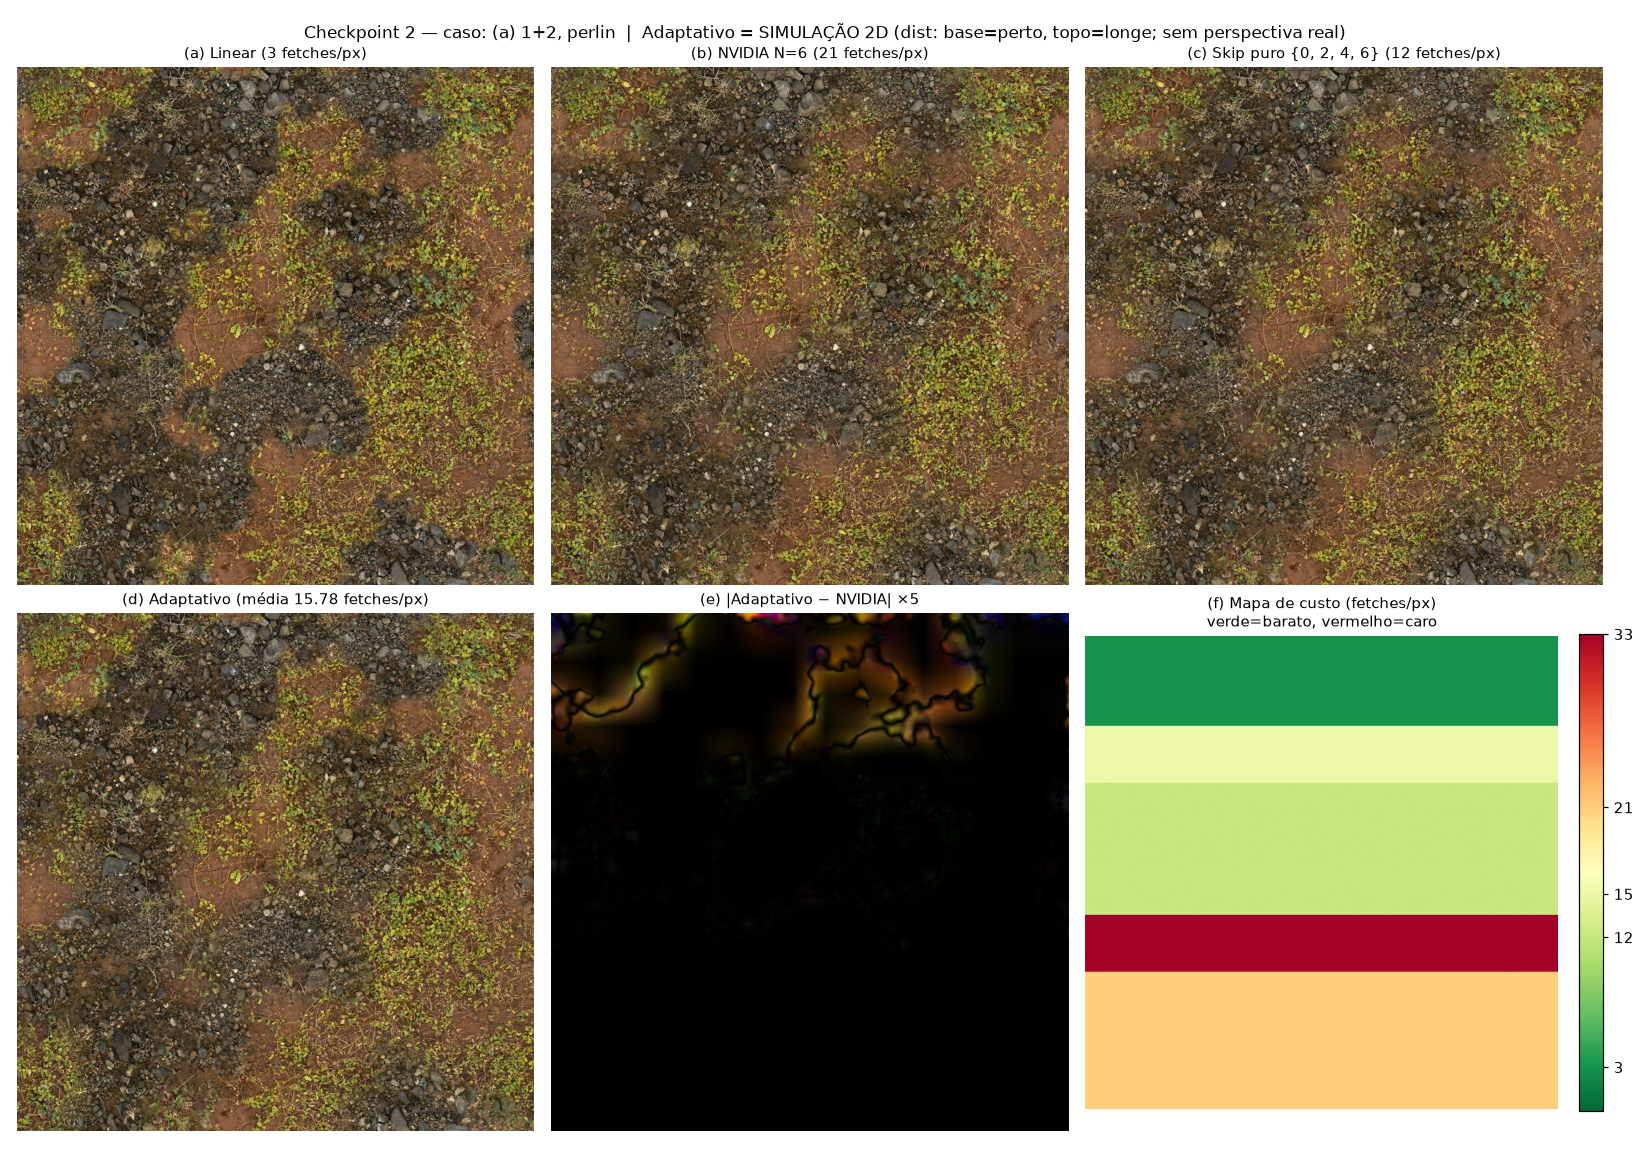
\includegraphics[width=0.96\textwidth]{../output/comparativo_checkpoint2.png}%
  }{%
    \fbox{\parbox{0.92\textwidth}{\centering\vspace{1.2cm}\small Painel Comparativo Visual (\texttt{../output/comparativo_checkpoint2.png}):\\ Linear Blending vs. NVIDIA 6 Níveis vs. \textit{Level Skipping} Puro/Híbrido vs. Adaptativo por Distância e Mapas de Erro Absoluto.\vspace{1.2cm}}}%
  }
  \caption{Comparação visual qualitativa e mapas de diferença absoluta amplificados ($5\times$) gerados pela bancada experimental do Checkpoint 2. O \textit{Linear Blending} exibe severo efeito fantasma (\textit{ghosting}) e perda de contraste na faixa central, enquanto o \textit{Level Skipping} Híbrido e o método Adaptativo por Distância preservam a nitidez das fissuras e a transição orgânica de cor com custo de amostragem significativamente reduzido.}
  \label{fig:comparativo_visual}
\end{figure*}

\subsection{Análise da Fronteira de Pareto e Adaptação por Distância}

A Figura~\ref{fig:comparativo_visual} ilustra os resultados visuais sobre os casos de teste, enquanto a Figura~\ref{fig:curva_pareto} apresenta a análise da fronteira de Pareto relacionando o custo de amostragem (\textit{texture fetches}/pixel) e a fidelidade de reconstrução (PSNR em dB). Verifica-se que as configurações de \textit{Level Skipping} Puro e Híbrido dominam rigorosamente toda a curva de truncamento simples, estabelecendo uma nova fronteira ótima custo-benefício.

No que tange ao \textbf{Esquema Adaptativo por Distância}, a formulação proposta transiciona continuamente entre os regimes operacionais através da ponderação hermítica com \texttt{smoothstep}. No benchmark bidimensional com gradiente de distância, o método atinge $\text{PSNR} = 38{,}69\text{ dB}$ e $\text{SSIM} = 0{,}9989$, com custo médio de $15{,}78$ fetches/px no somatório conservador das faixas de transição e $13{,}98$ fetches/px ao considerar a união e o reuso de leituras de textura compartilhadas ($-33{,}4\%$ vs. referência). Crucialmente, como a interpolação ocorre sobre os próprios pesos das máscaras ($G_{\alpha k}$) e não diretamente multiplicando as bandas fora de fase, a transição entre zonas não exibe qualquer artefato de descontinuidade temporal ou espacial (\textit{popping}), mesmo durante movimentação da câmera.

\begin{figure}[t]
  \centering
  \IfFileExists{../output/curva_pareto_custo_qualidade.png}{%
    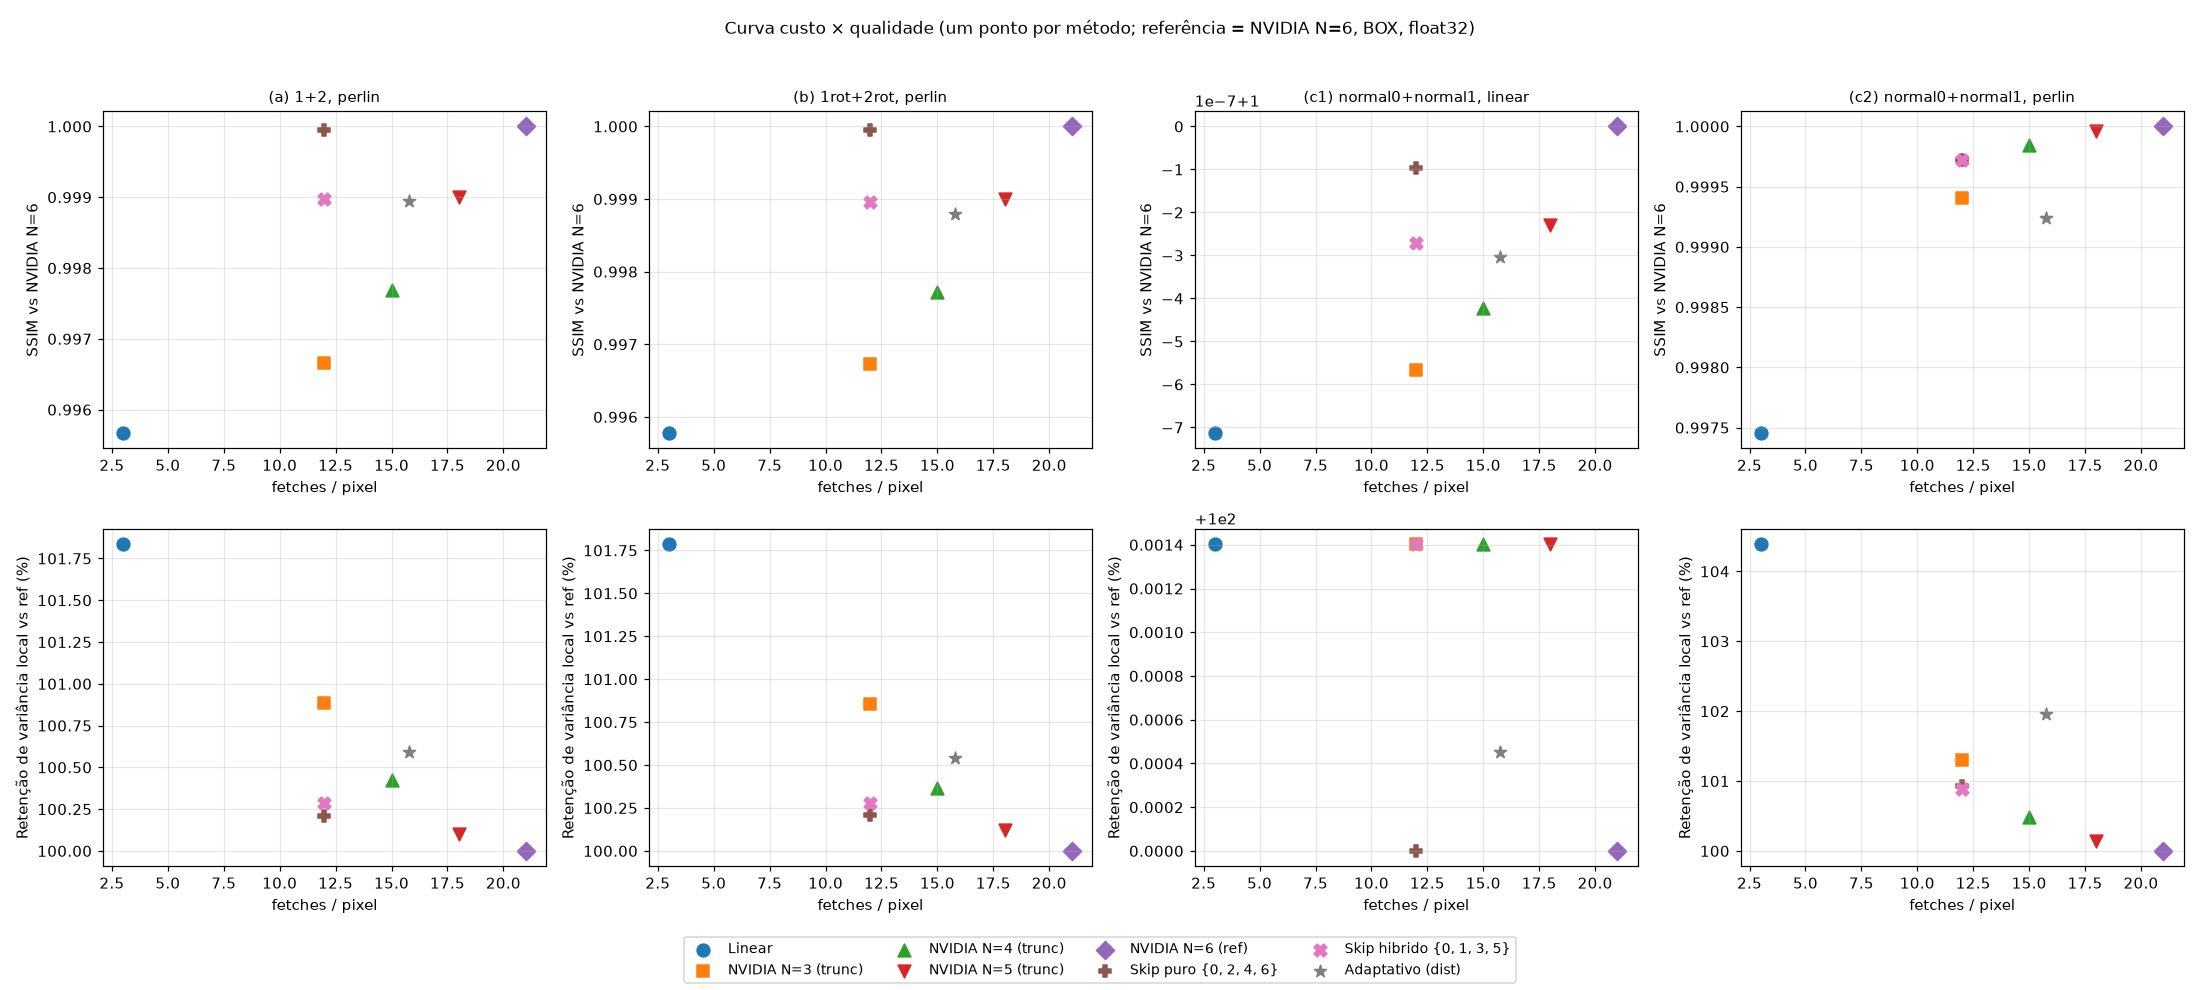
\includegraphics[width=0.98\columnwidth]{../output/curva_pareto_custo_qualidade.png}%
  }{%
    \fbox{\parbox{0.92\columnwidth}{\centering\vspace{1.0cm}\small Curva de Pareto Custo vs. Qualidade\\(\texttt{../output/curva_pareto_custo_qualidade.png})\vspace{1.0cm}}}%
  }
  \caption{Fronteira de Pareto relacionando o número de leituras de textura por fragmento (\textit{texture fetches}) e a qualidade de reconstrução (PSNR em dB). Nossas abordagens com \textit{Level Skipping} e adaptação contínua superam amplamente o truncamento simples de níveis de mesmo custo.}
  \label{fig:curva_pareto}
\end{figure}

\subsection{Impacto do Filtro de Reconstrução e Análise de Overshoot}

A Tabela~\ref{subtab:filtros} fornece a validação experimental do comportamento dos núcleos de decimação na formação da pirâmide Gaussiana. A decimação Box padrão de hardware serve como referência. O filtro Bilinear produz resultado quase idêntico em fidelidade ($48{,}24\text{ dB}$, $\text{SSIM} = 0{,}9999$) e taxa de \textit{overshoot} semelhante ($0{,}639\%$ vs. $0{,}633\%$).

Por outro lado, os filtros de maior suporte espacial que possuem lóbulos negativos no domínio espacial (Bicúbico e Lanczos) geram uma taxa substancialmente superior de valores extrapolados fora da faixa normalizada $[0, 1]$: $0{,}910\%$ de \textit{overshoot} para Bicúbico e $0{,}835\%$ para Lanczos, com valores mínimos caindo para $-0{,}082$ e máximos atingindo $1{,}101$. Embora o filtro Bicúbico ofereça discreto ganho numérico de nitidez ($51{,}45\text{ dB}$ contra a decimação Box), o impacto perceptivo em termos de SSIM é negligenciável ($1{,}0000$ vs. $0{,}9999$). O aumento na ocorrência de \textit{overshooting} exige compressão não-linear mais agressiva (\texttt{soft\_clip}) no fragment shader para evitar saturações espúrias. Conclui-se, portanto, que a decimação Box nativa de hardware da GPU combinada com interpolação bilinear de hardware para amostragem representa o ponto ideal de equilíbrio computacional e estabilidade numérica para renderização em tempo real.

% ============================================================================
\section{Dificuldades Encontradas, Limitações e Plano para Conclusão}
\label{sec:dificuldades}
% ============================================================================

\subsection{Dificuldades Técnicas Enfrentadas e Soluções Adotadas}

Durante o desenvolvimento e a validação experimental do Checkpoint 2, a equipe enfrentou e solucionou quatro desafios técnicos principais:
\begin{enumerate}
  \item \textbf{Ausência de \texttt{textureQueryLod} no perfil padrão WebGL 2.0 / GLSL ES 3.00:} diferentemente do OpenGL 4.0+ de desktop, o GLSL ES 3.00 utilizado pelo WebGL 2.0 não expõe a função intrínseca \texttt{textureQueryLod} para consultar diretamente o nível de \textit{mipmap} calculado pelo hardware. Solucionamos essa limitação implementando o estimador analítico exato baseado nas derivadas parciais de espaço de tela \texttt{dFdx} e \texttt{dFdy} escaladas pelas dimensões da textura (Equações~\eqref{eq:rho_footprint} e~\eqref{eq:lambda_lod}), garantindo portabilidade total entre navegadores e GPUs integradas ou dedicadas;
  \item \textbf{Descontinuidades visuais (\textit{popping}) na fronteira entre regimes de distância:} nas primeiras versões do protótipo adaptativo, a troca discreta (\texttt{if/else}) entre a pirâmide de 6 níveis e o \textit{Level Skipping} de 3 bandas gerava uma linha sutil de variação de contraste no terreno. Identificamos que multiplicar uma banda $L_k$ diretamente por um peso de atenuação violava a soma telescópica fora da zona de mistura. Resolucionamos o problema interpolando suavemente os \emph{pesos da máscara} entre escalas adjacentes via \texttt{smoothstep} ($\text{mix}(a_{k+2}, a_k, w_k)$), garantindo que a soma das bandas permaneça identicamente igual a $G_{x0}$ em regiões puras e eliminando totalmente o \textit{popping};
  \item \textbf{\textit{Overshooting} e artefatos de anelamento (\textit{ringing}) em filtros de suporte amplo:} ao testar o filtro de Lanczos ($a=2$) na bancada Python, os lóbulos negativos do núcleo $\text{sinc}$ acentuaram os picos das bandas Laplacianas, gerando valores fora de $[0, 1]$ em transições de alto contraste. A calibração da função de compressão não-linear \texttt{soft\_clip} centrada na média local $G_{\text{blend},K}$ (Equação~\eqref{eq:soft_clip}) suprimiu a saturação abrupta preservando o microcontraste;
  \item \textbf{Divergência de \textit{warps/wavefronts} em ramificações dinâmicas de GPU:} como as instruções \texttt{dFdx}/\texttt{dFdy} operam em blocos $2\times 2$, garantimos que o escalar de transição $\xi(\mathbf{p})$ varie suavemente no espaço de tela, mantendo alta coerência de execução entre \textit{threads} vizinhas da mesma unidade SIMD da GPU.
\end{enumerate}

\subsection{Limitações Atuais}

A principal limitação da abordagem atual reside no fato de que, na zona de transição estreita entre o regime de \textit{Level Skipping} e o regime de \textit{Linear Blending} ($\xi \in [0{,}65, 0{,}82]$), os fragmentos situados exatamente nessa faixa intermediária avaliam o \textit{Level Skipping} para permitir a interpolação suave antes do corte completo no horizonte ($\xi > 0{,}82$). Além disso, para materiais com anisotropia extrema vistos em ângulos rasantes (\textit{grazing angles}), o estimador isotrópico $\rho(\mathbf{p}) = \max(\|\partial_x \mathbf{w}\|, \|\partial_y \mathbf{w}\|)$ tende a superestimar o LOD na direção perpendicular à inclinação, o que motiva a investigação de adaptação anisotrópica na etapa final.

\subsection{Plano de Trabalho até a Entrega Final (29/11/2026)}

Para a conclusão do projeto e submissão da versão final do artigo e da apresentação em 29/11/2026, estabelecemos o seguinte cronograma de atividades:
\begin{itemize}
  \item \textbf{Semana 1 (12/11 a 18/11):} Integração de medição de tempo de GPU em tempo real via extensão \texttt{EXT\_disjoint\_timer\_query\_webgl2} no protótipo Three.js para reportar o tempo de quadro em milissegundos ($\text{ms}$) em diferentes resoluções (1080p e 4K);
  \item \textbf{Semana 2 (19/11 a 24/11):} Extensão do método adaptativo para considerar anisotropia elíptica em ângulos rasantes e inclusão de um cenário completo de terreno multi-material (3 camadas simultâneas com mapas de albedo, normal e rugosidade);
  \item \textbf{Semana 3 (25/11 a 29/11):} Consolidação dos gráficos definitivos de desempenho de hardware, revisão final do texto completo em LaTeX segundo as diretrizes da disciplina e gravação da demonstração interativa para a defesa final.
\end{itemize}

% ============================================================================
\bibliographystyle{plain}
\bibliography{referencias}
% ============================================================================

\end{document}
